\documentclass[a4paper]{article}
\usepackage[margin=1cm]{geometry}
\usepackage{amsmath, amssymb}
\usepackage{graphicx}
\usepackage{tikz}
\usetikzlibrary{arrows.meta}
\pagestyle{empty}

\definecolor{c0}{HTML}{E53935}
\definecolor{c1}{HTML}{1E88E5}
\definecolor{c2}{HTML}{43A047}
\definecolor{c3}{HTML}{FB8C00}
\definecolor{c4}{HTML}{8E24AA}
\definecolor{c5}{HTML}{00ACC1}
\definecolor{c6}{HTML}{F4511E}
\definecolor{c7}{HTML}{3949AB}
\definecolor{c8}{HTML}{7CB342}
\definecolor{c9}{HTML}{C2185B}
\definecolor{c10}{HTML}{FF7043}
\definecolor{c11}{HTML}{26A69A}
\definecolor{c12}{HTML}{5C6BC0}
\definecolor{c13}{HTML}{FFCA28}
\definecolor{c14}{HTML}{AB47BC}

\begin{document}

\begin{center}
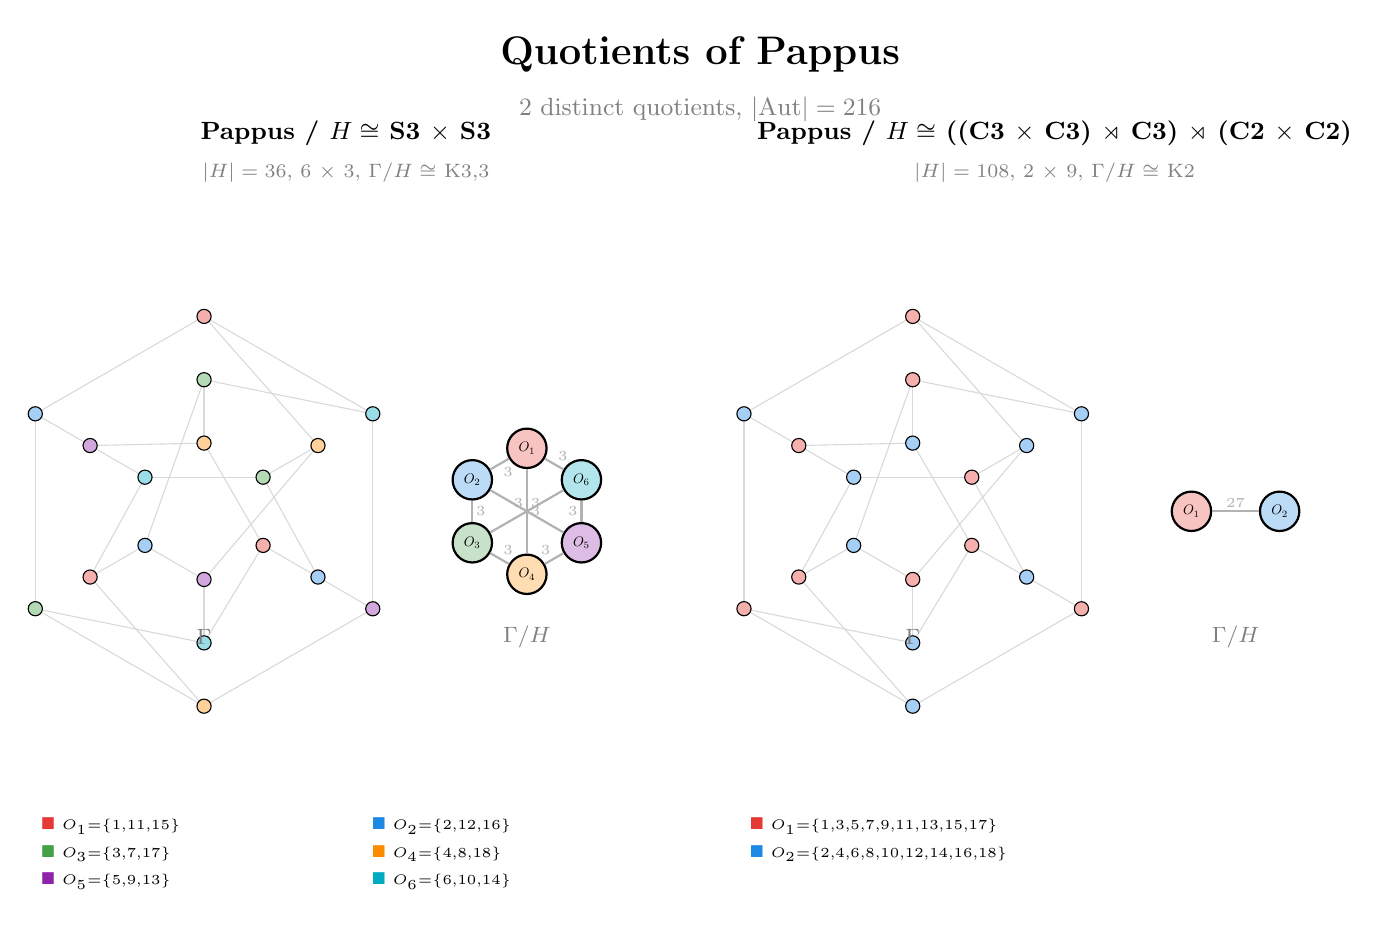
\begin{tikzpicture}[
  ov/.style={circle, draw, semithick, minimum size=3.5mm, inner sep=0pt},
  ovs/.style={circle, draw, thin, minimum size=1.8mm, inner sep=0pt},
  qv/.style={circle, draw, thick, minimum size=5mm, inner sep=0pt},
  cardtitle/.style={font=\small\bfseries},
  cardsub/.style={font=\scriptsize, text=gray},
  glabel/.style={font=\footnotesize, text=gray},
]
\node[font=\Large\bfseries] at (0, 11.5) {Quotients of Pappus};
\node[font=\small, text=gray] at (0, 10.8) {2 distinct quotients, $|\mathrm{Aut}|=216$};

% Card 1: H=S3 x S3
\node[cardtitle] at (-4.50,10.50) {Pappus / $H \cong$ S3 $\times$ S3};
\node[cardsub] at (-4.50,10.00) {$|H|=36$, 6 $\times$ 3, $\Gamma/H \cong$ K3,3};
\draw[gray!30, thin] (-6.300,8.175) -- (-8.443,6.938);
\draw[gray!30, thin] (-6.300,8.175) -- (-4.157,6.938);
\draw[gray!30, thin] (-6.300,8.175) -- (-4.853,6.535);
\draw[gray!30, thin] (-8.443,6.938) -- (-8.443,4.463);
\draw[gray!30, thin] (-8.443,6.938) -- (-7.747,6.535);
\draw[gray!30, thin] (-8.443,4.463) -- (-6.300,3.225);
\draw[gray!30, thin] (-8.443,4.463) -- (-6.300,4.029);
\draw[gray!30, thin] (-6.300,3.225) -- (-4.157,4.462);
\draw[gray!30, thin] (-6.300,3.225) -- (-7.747,4.865);
\draw[gray!30, thin] (-4.157,4.462) -- (-4.157,6.938);
\draw[gray!30, thin] (-4.157,4.462) -- (-4.853,4.865);
\draw[gray!30, thin] (-4.157,6.938) -- (-6.300,7.371);
\draw[gray!30, thin] (-6.300,7.371) -- (-6.300,6.566);
\draw[gray!30, thin] (-6.300,7.371) -- (-7.050,5.267);
\draw[gray!30, thin] (-6.300,6.566) -- (-7.747,6.535);
\draw[gray!30, thin] (-6.300,6.566) -- (-5.550,5.267);
\draw[gray!30, thin] (-7.747,6.535) -- (-7.050,6.133);
\draw[gray!30, thin] (-7.050,6.133) -- (-7.747,4.865);
\draw[gray!30, thin] (-7.050,6.133) -- (-5.550,6.133);
\draw[gray!30, thin] (-7.747,4.865) -- (-7.050,5.267);
\draw[gray!30, thin] (-7.050,5.267) -- (-6.300,4.834);
\draw[gray!30, thin] (-6.300,4.834) -- (-6.300,4.029);
\draw[gray!30, thin] (-6.300,4.834) -- (-4.853,6.535);
\draw[gray!30, thin] (-6.300,4.029) -- (-5.550,5.267);
\draw[gray!30, thin] (-5.550,5.267) -- (-4.853,4.865);
\draw[gray!30, thin] (-4.853,4.865) -- (-5.550,6.133);
\draw[gray!30, thin] (-5.550,6.133) -- (-4.853,6.535);
\node[ovs, fill=c0!40] at (-6.300,8.175) {};
\node[ovs, fill=c1!40] at (-8.443,6.938) {};
\node[ovs, fill=c2!40] at (-8.443,4.463) {};
\node[ovs, fill=c3!40] at (-6.300,3.225) {};
\node[ovs, fill=c4!40] at (-4.157,4.462) {};
\node[ovs, fill=c5!40] at (-4.157,6.938) {};
\node[ovs, fill=c2!40] at (-6.300,7.371) {};
\node[ovs, fill=c3!40] at (-6.300,6.566) {};
\node[ovs, fill=c4!40] at (-7.747,6.535) {};
\node[ovs, fill=c5!40] at (-7.050,6.133) {};
\node[ovs, fill=c0!40] at (-7.747,4.865) {};
\node[ovs, fill=c1!40] at (-7.050,5.267) {};
\node[ovs, fill=c4!40] at (-6.300,4.834) {};
\node[ovs, fill=c5!40] at (-6.300,4.029) {};
\node[ovs, fill=c0!40] at (-5.550,5.267) {};
\node[ovs, fill=c1!40] at (-4.853,4.865) {};
\node[ovs, fill=c2!40] at (-5.550,6.133) {};
\node[ovs, fill=c3!40] at (-4.853,6.535) {};
\node[glabel] at (-6.30,4.10) {$\Gamma$};
\node[qv, fill=c0!30] (c0o0) at (-2.200,6.500) {\scalebox{0.5}{$O_{1}$}};
\node[qv, fill=c1!30] (c0o1) at (-2.893,6.100) {\scalebox{0.5}{$O_{2}$}};
\node[qv, fill=c2!30] (c0o2) at (-2.893,5.300) {\scalebox{0.5}{$O_{3}$}};
\node[qv, fill=c3!30] (c0o3) at (-2.200,4.900) {\scalebox{0.5}{$O_{4}$}};
\node[qv, fill=c4!30] (c0o4) at (-1.507,5.300) {\scalebox{0.5}{$O_{5}$}};
\node[qv, fill=c5!30] (c0o5) at (-1.507,6.100) {\scalebox{0.5}{$O_{6}$}};
\draw[gray!60, thick] (c0o0) -- node[font=\tiny, auto, inner sep=1pt] {3} (c0o1);
\draw[gray!60, thick] (c0o0) -- node[font=\tiny, auto, inner sep=1pt] {3} (c0o3);
\draw[gray!60, thick] (c0o0) -- node[font=\tiny, auto, inner sep=1pt] {3} (c0o5);
\draw[gray!60, thick] (c0o1) -- node[font=\tiny, auto, inner sep=1pt] {3} (c0o2);
\draw[gray!60, thick] (c0o1) -- node[font=\tiny, auto, inner sep=1pt] {3} (c0o4);
\draw[gray!60, thick] (c0o2) -- node[font=\tiny, auto, inner sep=1pt] {3} (c0o3);
\draw[gray!60, thick] (c0o2) -- node[font=\tiny, auto, inner sep=1pt] {3} (c0o5);
\draw[gray!60, thick] (c0o3) -- node[font=\tiny, auto, inner sep=1pt] {3} (c0o4);
\draw[gray!60, thick] (c0o4) -- node[font=\tiny, auto, inner sep=1pt] {3} (c0o5);
\node[glabel] at (-2.20,4.10) {$\Gamma/H$};
\node[anchor=west, font=\tiny] at (-8.50,1.70) {\textcolor{c0}{$\blacksquare$} $O_{1}$=\{1,11,15\}};
\node[anchor=west, font=\tiny] at (-4.30,1.70) {\textcolor{c1}{$\blacksquare$} $O_{2}$=\{2,12,16\}};
\node[anchor=west, font=\tiny] at (-8.50,1.35) {\textcolor{c2}{$\blacksquare$} $O_{3}$=\{3,7,17\}};
\node[anchor=west, font=\tiny] at (-4.30,1.35) {\textcolor{c3}{$\blacksquare$} $O_{4}$=\{4,8,18\}};
\node[anchor=west, font=\tiny] at (-8.50,1.00) {\textcolor{c4}{$\blacksquare$} $O_{5}$=\{5,9,13\}};
\node[anchor=west, font=\tiny] at (-4.30,1.00) {\textcolor{c5}{$\blacksquare$} $O_{6}$=\{6,10,14\}};

% Card 2: H=((C3 x C3) : C3) : (C2 x C2)
\node[cardtitle] at (4.50,10.50) {Pappus / $H \cong$ ((C3 $\times$ C3) $\rtimes$ C3) $\rtimes$ (C2 $\times$ C2)};
\node[cardsub] at (4.50,10.00) {$|H|=108$, 2 $\times$ 9, $\Gamma/H \cong$ K2};
\draw[gray!30, thin] (2.700,8.175) -- (0.557,6.938);
\draw[gray!30, thin] (2.700,8.175) -- (4.843,6.938);
\draw[gray!30, thin] (2.700,8.175) -- (4.147,6.535);
\draw[gray!30, thin] (0.557,6.938) -- (0.557,4.463);
\draw[gray!30, thin] (0.557,6.938) -- (1.253,6.535);
\draw[gray!30, thin] (0.557,4.463) -- (2.700,3.225);
\draw[gray!30, thin] (0.557,4.463) -- (2.700,4.029);
\draw[gray!30, thin] (2.700,3.225) -- (4.843,4.462);
\draw[gray!30, thin] (2.700,3.225) -- (1.253,4.865);
\draw[gray!30, thin] (4.843,4.462) -- (4.843,6.938);
\draw[gray!30, thin] (4.843,4.462) -- (4.147,4.865);
\draw[gray!30, thin] (4.843,6.938) -- (2.700,7.371);
\draw[gray!30, thin] (2.700,7.371) -- (2.700,6.566);
\draw[gray!30, thin] (2.700,7.371) -- (1.950,5.267);
\draw[gray!30, thin] (2.700,6.566) -- (1.253,6.535);
\draw[gray!30, thin] (2.700,6.566) -- (3.450,5.267);
\draw[gray!30, thin] (1.253,6.535) -- (1.950,6.133);
\draw[gray!30, thin] (1.950,6.133) -- (1.253,4.865);
\draw[gray!30, thin] (1.950,6.133) -- (3.450,6.133);
\draw[gray!30, thin] (1.253,4.865) -- (1.950,5.267);
\draw[gray!30, thin] (1.950,5.267) -- (2.700,4.834);
\draw[gray!30, thin] (2.700,4.834) -- (2.700,4.029);
\draw[gray!30, thin] (2.700,4.834) -- (4.147,6.535);
\draw[gray!30, thin] (2.700,4.029) -- (3.450,5.267);
\draw[gray!30, thin] (3.450,5.267) -- (4.147,4.865);
\draw[gray!30, thin] (4.147,4.865) -- (3.450,6.133);
\draw[gray!30, thin] (3.450,6.133) -- (4.147,6.535);
\node[ovs, fill=c0!40] at (2.700,8.175) {};
\node[ovs, fill=c1!40] at (0.557,6.938) {};
\node[ovs, fill=c0!40] at (0.557,4.463) {};
\node[ovs, fill=c1!40] at (2.700,3.225) {};
\node[ovs, fill=c0!40] at (4.843,4.462) {};
\node[ovs, fill=c1!40] at (4.843,6.938) {};
\node[ovs, fill=c0!40] at (2.700,7.371) {};
\node[ovs, fill=c1!40] at (2.700,6.566) {};
\node[ovs, fill=c0!40] at (1.253,6.535) {};
\node[ovs, fill=c1!40] at (1.950,6.133) {};
\node[ovs, fill=c0!40] at (1.253,4.865) {};
\node[ovs, fill=c1!40] at (1.950,5.267) {};
\node[ovs, fill=c0!40] at (2.700,4.834) {};
\node[ovs, fill=c1!40] at (2.700,4.029) {};
\node[ovs, fill=c0!40] at (3.450,5.267) {};
\node[ovs, fill=c1!40] at (4.147,4.865) {};
\node[ovs, fill=c0!40] at (3.450,6.133) {};
\node[ovs, fill=c1!40] at (4.147,6.535) {};
\node[glabel] at (2.70,4.10) {$\Gamma$};
\node[qv, fill=c0!30] (c1o0) at (6.240,5.700) {\scalebox{0.5}{$O_{1}$}};
\node[qv, fill=c1!30] (c1o1) at (7.360,5.700) {\scalebox{0.5}{$O_{2}$}};
\draw[gray!60, thick] (c1o0) -- node[font=\tiny, auto, inner sep=1pt] {27} (c1o1);
\node[glabel] at (6.80,4.10) {$\Gamma/H$};
\node[anchor=west, font=\tiny] at (0.50,1.70) {\textcolor{c0}{$\blacksquare$} $O_{1}$=\{1,3,5,7,9,11,13,15,17\}};
\node[anchor=west, font=\tiny] at (0.50,1.35) {\textcolor{c1}{$\blacksquare$} $O_{2}$=\{2,4,6,8,10,12,14,16,18\}};
\end{tikzpicture}
\end{center}

\end{document}